Plusieurs pièces mécaniques ont dû être développées pendant ce projet comme par exemple le support de pieds  qui a déjà été décrit au chapitre \ref{sec:DescStruct}.
Maintenant que les éléments sont en place, il faut les lier ensemble avec des pièces faites sur mesure. Toutes les pièces sont faites
d'aluminium EN-AW 6082 sauf si mentionné autrement. Les dimensions indiquées sur les figures sont en mm sauf si mentionné autrement.

\section{Assemblage mécanique complet}\label{sec:AssMecComp}
L'assemblage de toutes les pièces mécaniques fabriquées avec la structure et les composants commandés vu de face et de derrière est
donné ci-dessous. Cette image permet de donner une idée d'où sont placées les pièces qui seront discutées plus loin dans ce chapitre. Une vue
éclatée d'une partie du système est aussi disponible dans l'annexe B.

\begin{figure}[H]
    \centering
    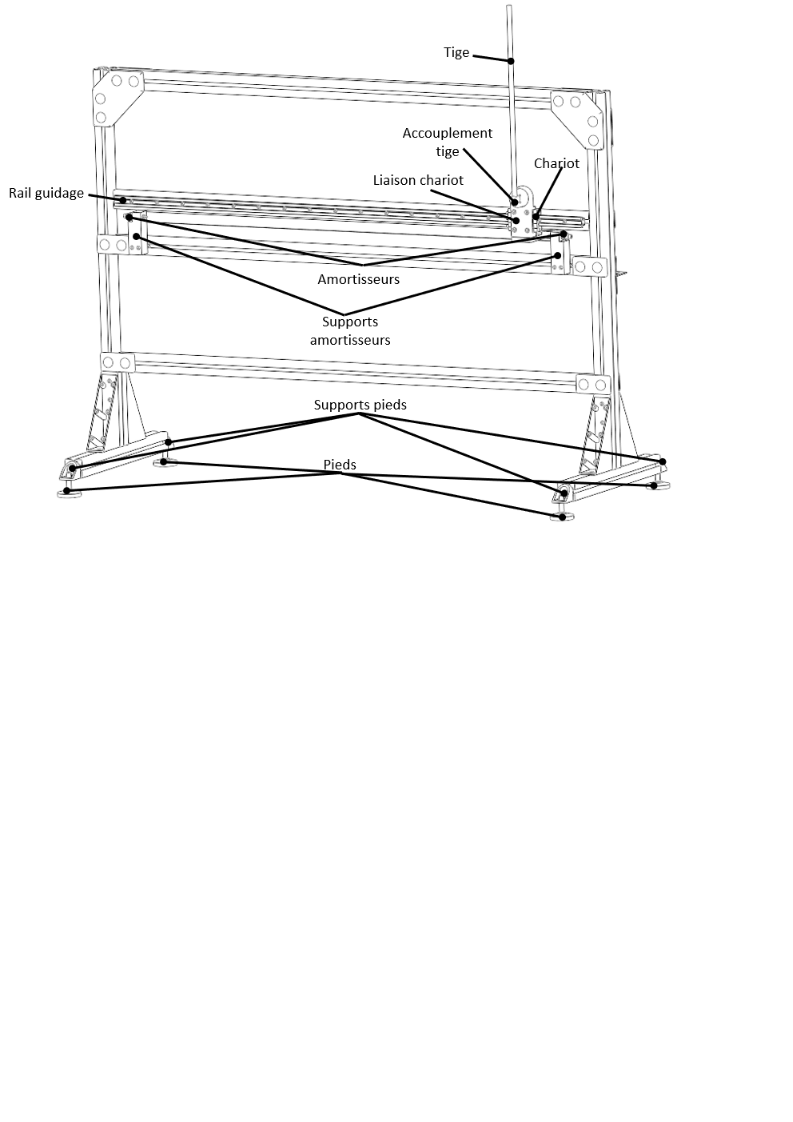
\includegraphics[width = 0.9\textwidth]{assets/figures/AssemblageCompletFace.svg}
    \caption{Représentation de l'assemblage mécanique complet vu de face}
    \label{fig:AssCompFace}
\end{figure}

\begin{figure}[H]
    \centering
    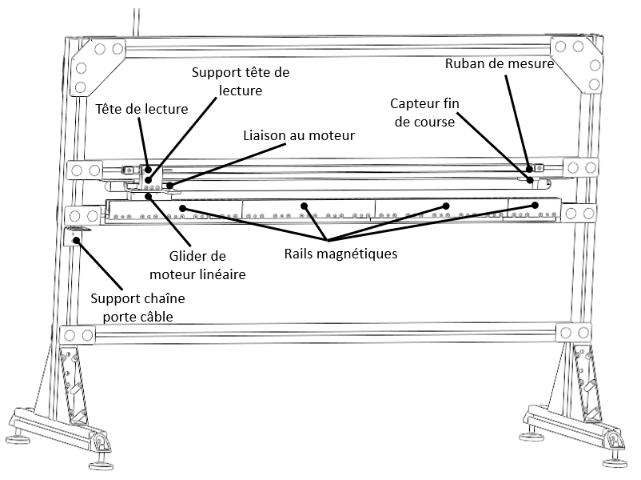
\includegraphics[width = 0.9\textwidth]{assets/figures/AssemblageCompletDerriere.svg}
    \caption{Représentation de l'assemblage mécanique complet vu de derrière}
    \label{fig:AssCompDerriere}
\end{figure}

\section{Liaison Moteur-Glider}\label{sec:LiaisonMotGlid}
La liaison entre le chariot du guidage et le \gls{glider} du moteur va se faire en deux pièces vissées ensemble. L'assemblage de ces pièces
entre elles et avec leurs liaisons directes donne la mise en plan suivante.

\begin{figure}[H]
    \centering
    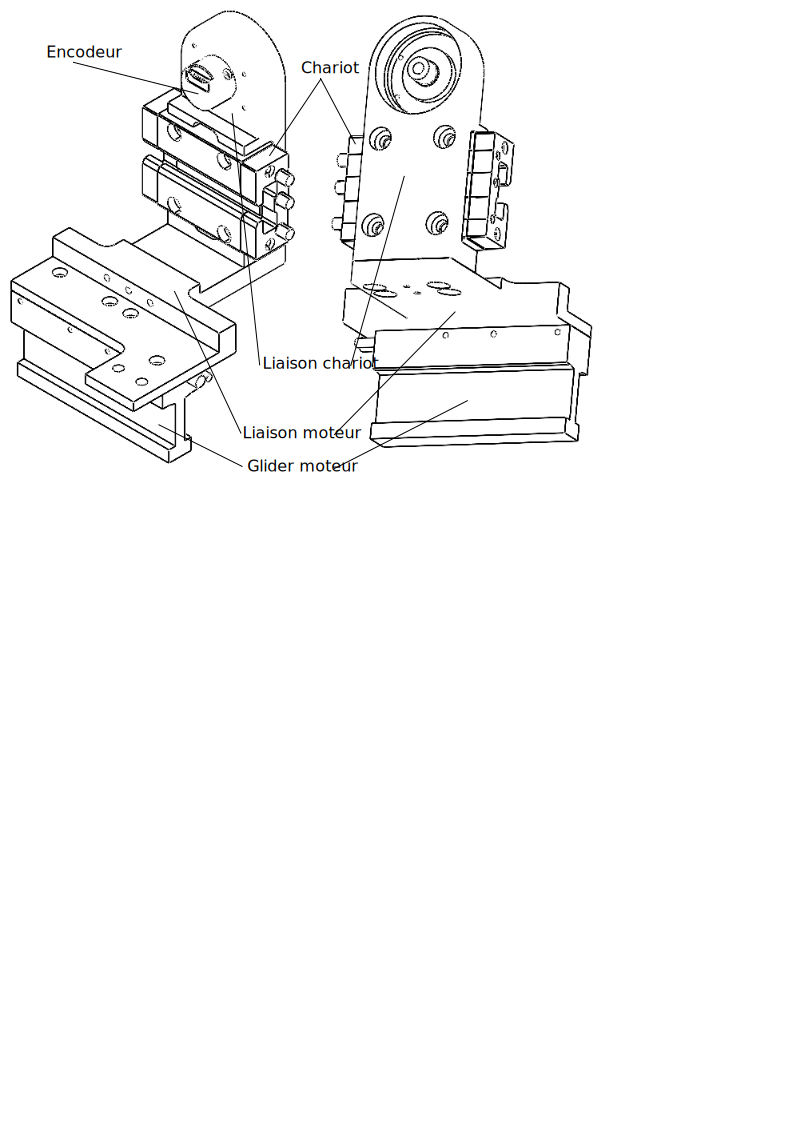
\includegraphics[width = 0.8\textwidth]{assets/figures/AssemblageGuidageEntrainement.svg}
    \caption{Représentation de l'assemblage des pièces de guidage et d'entrainement du système}
    \label{fig:AssGuiEntr}
\end{figure}

La première pièce, la liaison au chariot, est illustrée sur l'image suivante.

\begin{figure}[H]
    \centering
    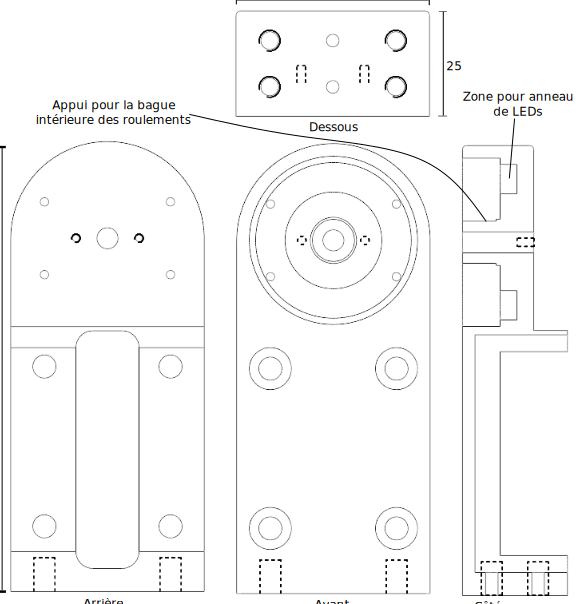
\includegraphics[width = 0.6\textwidth]{assets/figures/LiaisonChariot.svg}
    \caption{Représentation de la pièce de liaison du chariot}
    \label{fig:LiaisonChariot}
\end{figure}

La liaison au chariot devra accueillir deux roulements rigides à billes qui servent à faire tourner la partie qui tient la tige du pendule. Une tolérance
h6 est présente sur le diamètre intérieur pour les roulements en suivant les spécifications des normes \cite{Ajustements}. Une zone pour placer
un anneau de LEDs est aussi nécessaire afin de pouvoir illuminer la tige. Enfin, cette pièce devra aussi accueillir l'encodeur pour la position
angulaire. Une fente sur l'arrière est prévue pour le passage de câble des LEDs et de l'encodeur. La fixation sur le chariot se fait avec quatre
vis M5 ce qui nécessitera donc des lamages sur la face avant. La fixation sur l'autre pièce se fait sur le dessous avec quatre taraudages M5.
Deux alésages sont présents avec une tolérance H7 pour des goupilles qui permettent l'indexage avec la liaison moteur.\\

La seconde pièce, la liaison moteur, devra évidemment se lier avec la première, mais aussi avec le moteur. Elle est représentée sur l'illustration
suivante.

\begin{figure}[H]
    \centering
    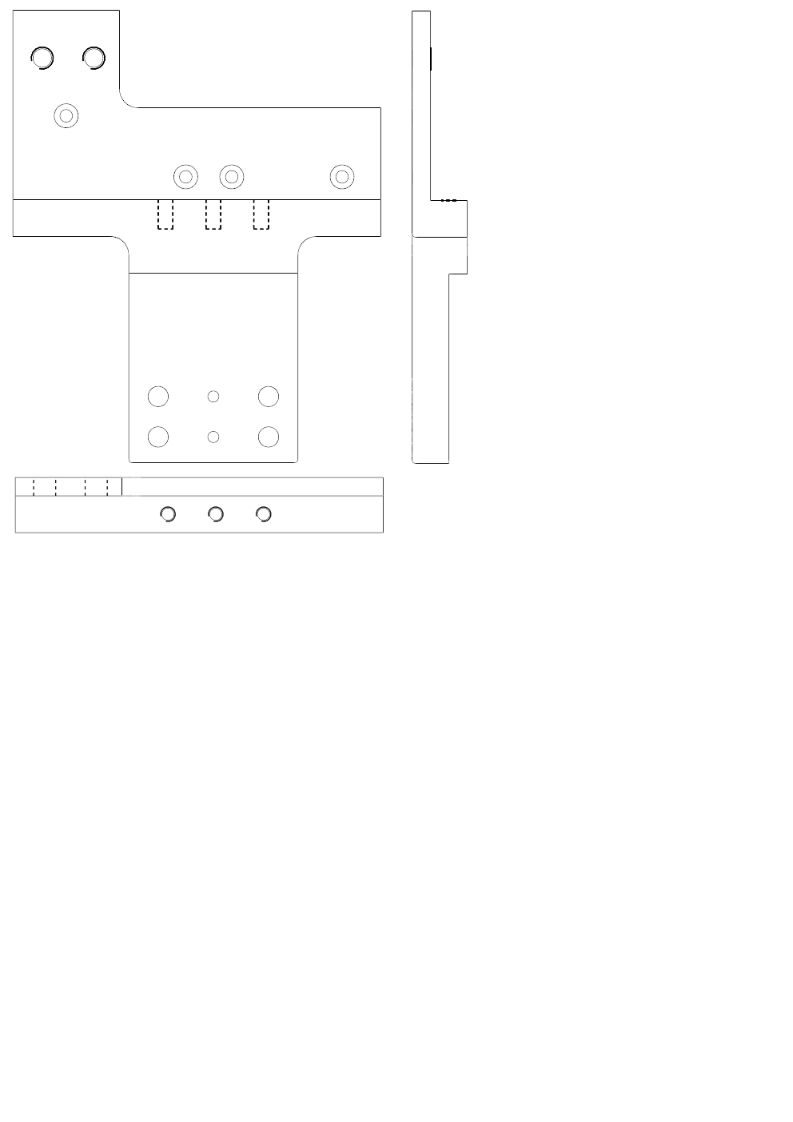
\includegraphics[width = 0.5\textwidth]{assets/figures/LiaisonMoteur.svg}
    \caption{Représentation de la pièce de liaison du moteur}
    \label{fig:LiaisonMoteur}
\end{figure}

La première pièce ayant les taraudages, celle-ci aura quatre passages de vis M5 ainsi que deux trous avec la tolérance K7 pour les goupilles d'indexage
sur le dessus.
Pour la fixation au moteur, quatre lamages M3 placés sur le dessus suffiront. Deux autres éléments viennent encore se fixer sur cette pièce: le support de la tête de
lecture pour la règle linéaire et la chaîne porte-câbles. Pour le support de tête de lecture, trois taraudages M4 sont placés sur la face avant, alors
que deux trous taraudés M6 sur le dessus sont utilisés pour fixer la chaîne porte-câbles.

\section{Support tête de lecture}\label{sec:SupTeteLect}
Le support de la tête de lecture de la règle linéaire est fixé sur la liaison au moteur comme mentionné plus haut. Ci-dessous, une représentation
avec le support monté sur la liaison au moteur et avec la tête de lecture.

\begin{figure}[H]
    \centering
    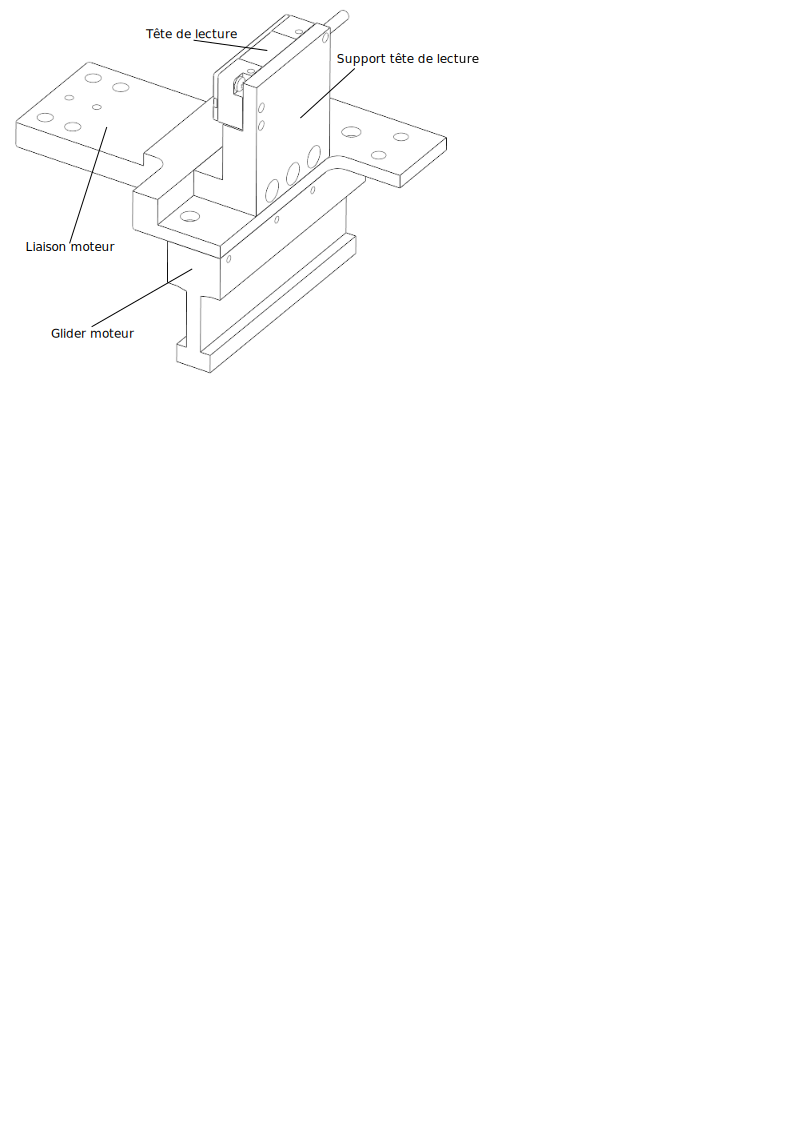
\includegraphics[width = 0.6\textwidth]{assets/figures/AssemblageMesureLineaire.svg}
    \caption{Représentation du support de tête de lecture assemblée avec les pièces proches dans le système}
    \label{fig:AssMesLin}
\end{figure}

Trois lamages M4 pour se fixer à la liaison moteur ainsi que deux trous de passage pour vis M3 pour la tête de lecture sont présents sur la face
avant. Un trou supplémentaire est ajouté sur cette face pour faire le réglage en position de la tête. La pièce obtenue est la suivante.

\begin{figure}[H]
    \centering
    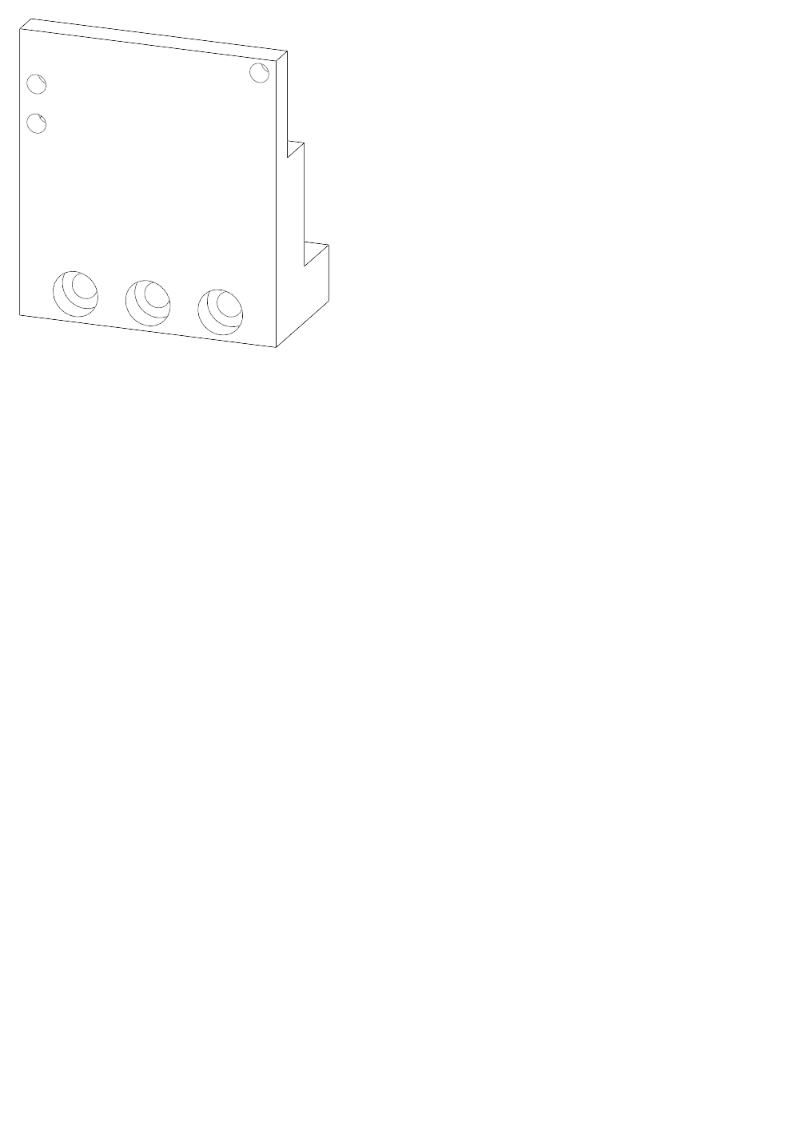
\includegraphics[width = 0.4\textwidth]{assets/figures/SupportTeteLecture.svg}
    \caption{Représentation du support de tête de lecture}
    \label{fig:SupTeteLect}
\end{figure}

\section{Support amortisseur}\label{sec:SupAmort}
Les amortisseurs se trouvent à l'avant du système au bout de chaque côté de la course. Le placement des supports de l'amortisseur sur un des
côtés est visible sur cette image.

\begin{figure}[H]
    \centering
    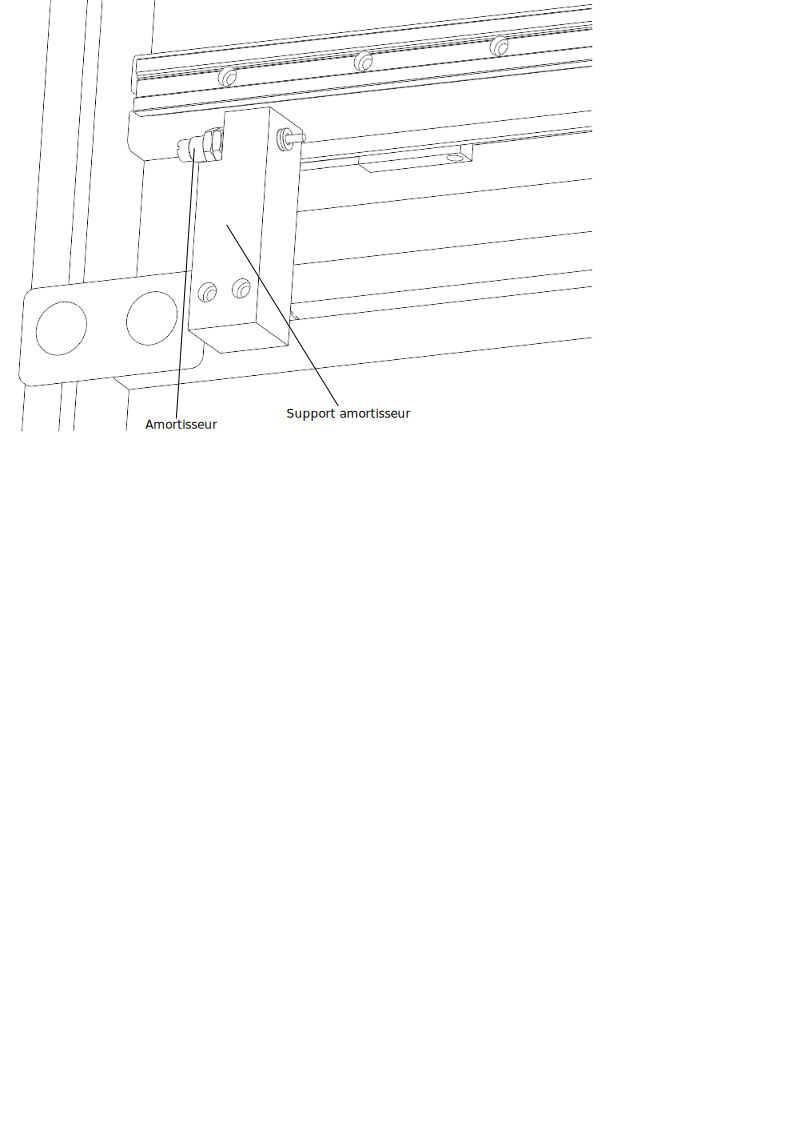
\includegraphics[width = 0.8\textwidth]{assets/figures/PlacementSupports.svg}
    \caption{Représentation du placement de l'amortisseur pour un côté}
    \label{fig:PlaceSup}
\end{figure}

Leur support doit être assez épais pour pouvoir supporter les chocs. Un trou de passage M10 est nécessaire pour fixer l'amortisseur et deux
lamages M4 permettent la fixation sur le profilé. Les deux amortisseurs étant dans des directions opposées, il faut créer deux supports
symétriques pour pouvoir les fixer. La représentation d'un des supports se trouve ci-dessous.

\begin{figure}[H]
    \centering
    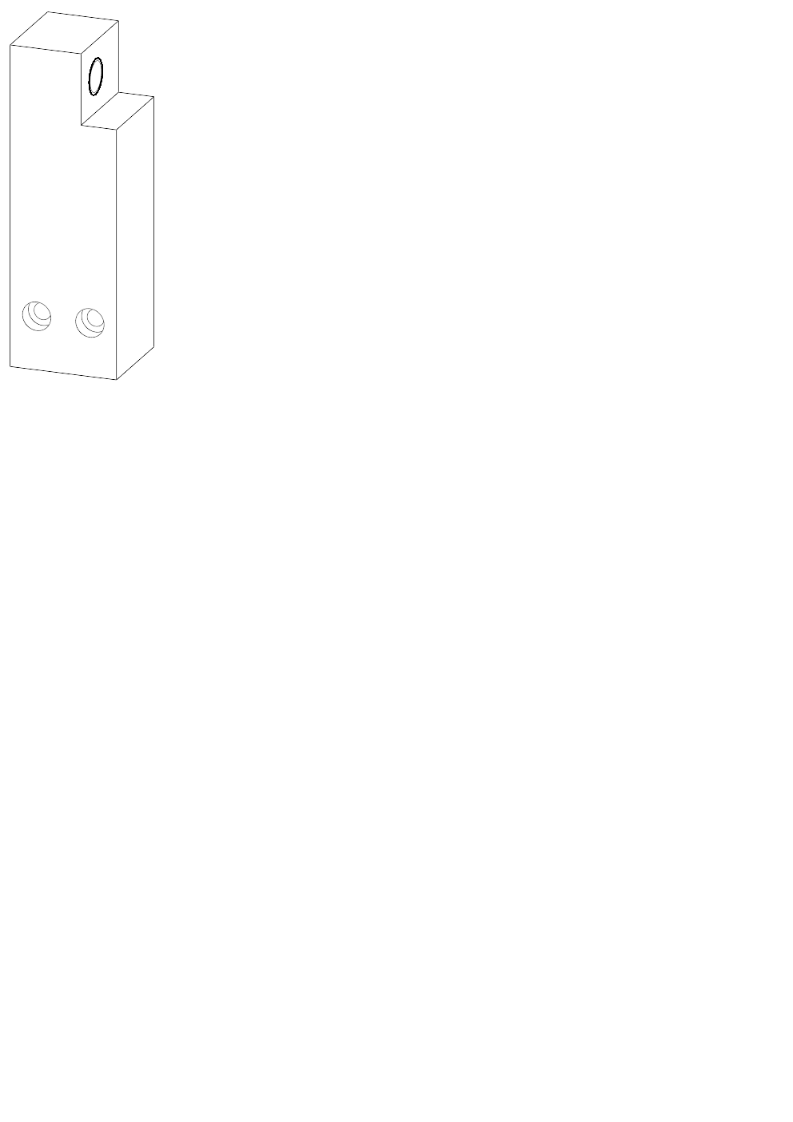
\includegraphics[width = 0.2\textwidth]{assets/figures/SupportAmortisseur.svg}
    \caption{Représentation du support de l'amortisseur}
    \label{fig:SupAmort}
\end{figure}

\section{Partie tournante}\label{sec:PartieTour}
La partie tournante du système est composée de plusieurs pièces, dont deux en polycarbonate transparent. L'assemblage de ces différentes pièces ainsi que de
la liaison au chariot et l'encodeur donne la représentation suivante.

\begin{figure}[H]
    \centering
    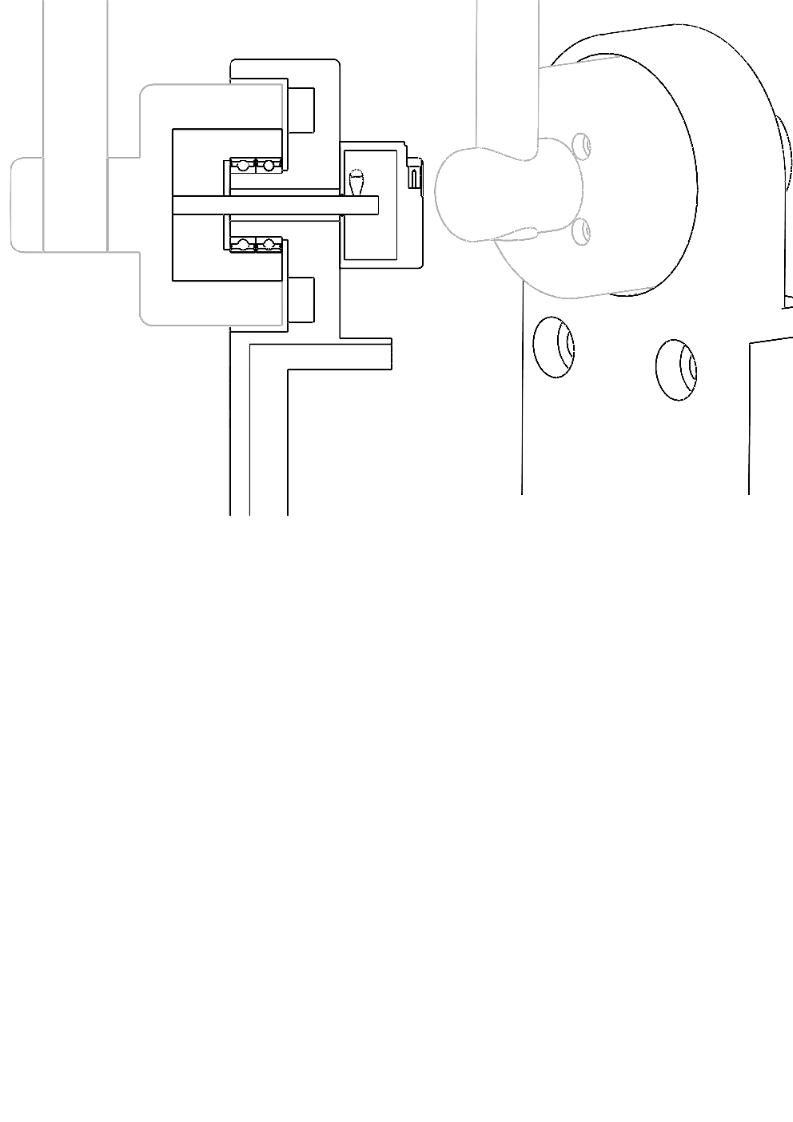
\includegraphics[width = 0.7\textwidth]{assets/figures/AssemblagePartieTournante.svg}
    \caption{Représentation de l'assemblage des parties tournantes et leurs connections directes}
    \label{fig:AssPartieTour}
\end{figure}

Tout d'abord, la partie en contact direct avec les roulements et qui fait tourner l'encodeur angulaire, le couplage encodeur. Cette partie est
faites en 2 morceaux qui sont chassés ensemble et est aussi attachée à une autre pièce, le couplage à la tige, à l'aide de quatre taraudages M2.
La première partie de la pièce, couplage encodeur 1, est illustrée ci-après.

\begin{figure}[H]
    \centering
    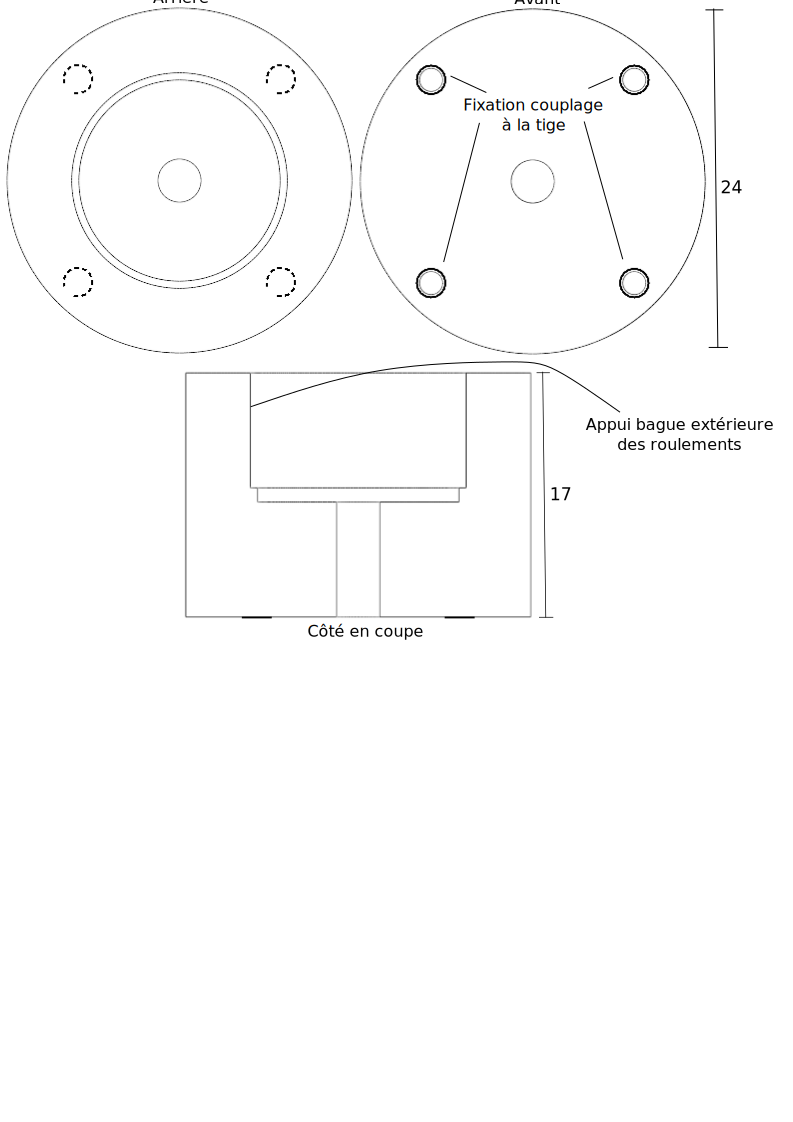
\includegraphics[width = 0.9\textwidth]{assets/figures/CouplageEncodeur.svg}
    \caption{Représentation du couplage à l'encodeur}
    \label{fig:CouplEnco}
\end{figure}

La seconde partie, couplage encodeur 2, qui vient se chasser dans le trou central de la première est un arbre rectifié de 3~mm de diamètre et 32~mm
de long en acier CK45.

Le couplage encodeur et le couplage à la tige sont imbriqués l'un dans l'autre et il faut donc une tolérance sur le diamètre extérieur du couplage encodeur de h6. Il faut aussi mettre une tolérance
sur le diamètre intérieur qui définit la face où s'appuye les roulements donc une tolérance de M7 a été choisie car la bague extérieure du
roulement est fixe par rapport aux efforts et ceux-ci sont faibles \cite{Ajustements}.

La pièce de couplage à la tige qui est attachée à celle montrée sur la figure \ref{fig:CouplEnco} est en \acrshort{PC}. La pièce est illustré à
l'image suivante.

\begin{figure}[H]
    \centering
    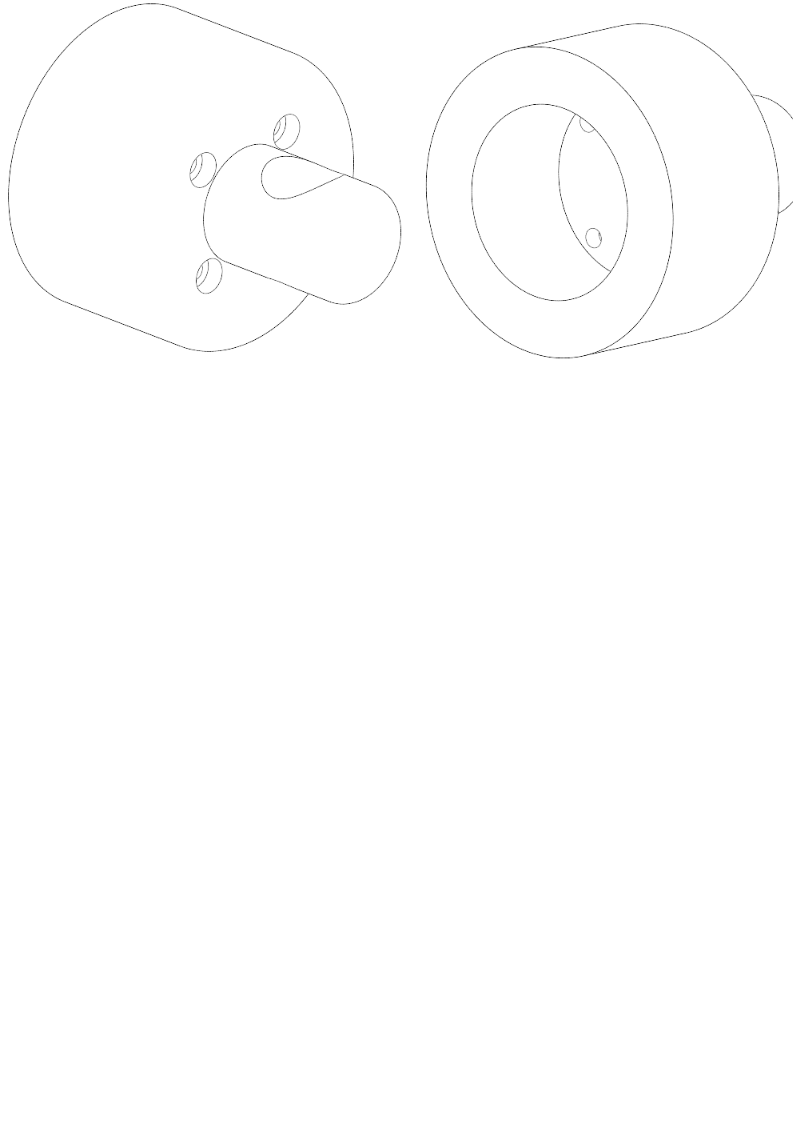
\includegraphics[width = 0.7\textwidth]{assets/figures/CouplageTige.svg}
    \caption{Représentation du couplage à la tige}
    \label{fig:CouplTige}
\end{figure}

Elle possède donc quatre lamages M2 pour pouvoir se visser sur le couplage encodeur et aussi un perçage de 10~mm de diamètre ajusté avec la tige
qui sera chassée dedans. Une tolérance H7 est présente sur le diamètre intérieur de la pièce pour avoir un jeu incertain avec la pièce de
couplage à l'encodeur.

La tige, elle aussi en \acrshort{PC}, vient se placer dans le perçage de 10~mm de la pièce précédente. La tige a donc un
diamètre lui aussi égal à 10~mm et une longueur de 420~mm. Aucune autre modification n'est apportée à la tige à part un chanfrein afin d'éviter
les arêtes coupantes.\\

Les forces qui s'appliquent aux roulements peuvent maintenant être calculées à l'aide du schéma de forces sur la figure \ref{fig:CalcRoul}.
Les termes utilisés dans ce schéma sont les suivants:

\begin{table}[H]
    \centering
    \caption{Valeurs utilisées pour les calculs}
    \label{tab:ValCalcRoul}
    \begin{tabular}{|l|l|l|l|}
        \hline
        \textbf{Donnée}                        & \textbf{Lettre} & \textbf{Valeur} & \textbf{Unité} \\ \hline
        Masse de la tige                       & $m_T$           & 39              & $g$            \\ \hline
        Masse du couplage à la tige            & $m_{CT}$        & 23              & $g$            \\ \hline
        Masse du couplage à l'encodeur 1       & $m_{CE1}$       & 16              & $g$            \\ \hline
        Masse du couplage à l'encodeur 2       & $m_{CE2}$       & 2               & $g$            \\ \hline
        Accélération de la pesanteur sur Terre & $g$             & 9.81            & $m/s^2$        \\ \hline
        Force radiale sur le roulement 1       & $F_{R1}$        & ?               & $N$            \\ \hline
        Force radiale sur le roulement 2       & $F_{R2}$        & ?               & $N$            \\ \hline
        Distance de $m_{CE2}$ à A              & $d_1$           & 1               & $mm$           \\ \hline
        Distance de $F_{R1}$ à A               & $d_2$           & 4               & $mm$           \\ \hline
        Distance de $m_{CE1}$ à A              & $d_3$           & 7.5             & $mm$           \\ \hline
        Distance de $m_{CT}$ à A               & $d_4$           & 12.5            & $mm$           \\ \hline
        Distance de $m_{T}$ à A                & $d_5$           & 30              & $mm$           \\ \hline
    \end{tabular}%
\end{table}

\begin{figure}[H]
    \centering
    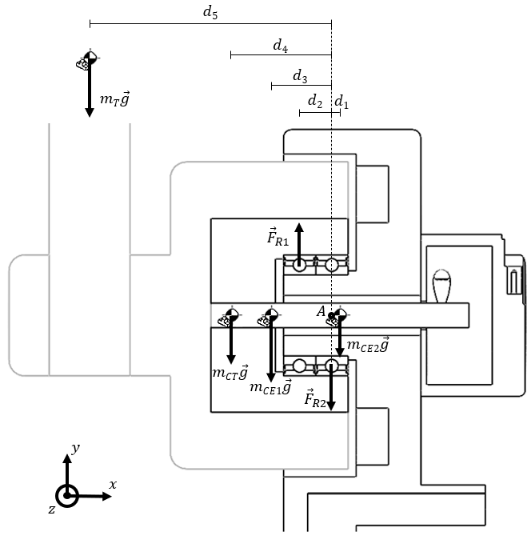
\includegraphics[width = 0.8\textwidth]{assets/figures/CalculRoulements.svg}
    \caption{Schéma de forces pour le calcul des efforts appliqués sur les roulements}
    \label{fig:CalcRoul}
\end{figure}

Les formules suivantes peuvent être tirées à partir du schéma dans le but d'obtenir les valeurs de $F_{R1}$ et $F_{R2}$.\\
Somme des moments de forces pour pièces statiques autour du point A:

\begin{equation}
    \begin{aligned}
         & \Sigma \vec{M}_A = 0                                                                                                                                                       \\
         & \Rightarrow  m_T \cdot \vec{g} \cdot d_5 + m_{CT} \cdot \vec{g} \cdot d_4 + m_{CE1} \cdot \vec{g} \cdot d_3 - m_{CE2} \cdot \vec{g} \cdot d_1 - \vec{F}_{R1} \cdot d_2 = 0 \\
         & \Rightarrow  \vec{F}_{R1} = \vec{g} \cdot \frac{m_T \cdot d_5 + m_{CT} \cdot d_4 + m_{CE1} \cdot d_3 - m_{CE2} \cdot d_1}{d_2}                                             \\
         & = 9.81 \cdot \frac{0.039 \cdot 0.03 + 0.023 \cdot 0.0125 + 0.016 \cdot 0.0075 - 0.002 \cdot 0.001}{0.004} = 3.9~N
    \end{aligned}
\end{equation}

Somme des forces sur l'axe y pour pièces statiques:

\begin{equation}
    \begin{aligned}
         & \Sigma \vec{F}_y = 0 \Rightarrow \vec{F}_{R1} - \vec{F}_{R2} - m_T \cdot \vec{g} - m_{CT} \cdot \vec{g} - m_{CE1} \cdot \vec{g} - m_{CE2} \cdot \vec{g} = 0 \\
         & \Rightarrow \vec{F}_{R2} = \vec{F}_{R1} - \vec{g} \cdot (m_T + m_{CT} + m_{CE1} + m_{CE2})                                                                  \\
         & = 3.9 - 9.81 \cdot (0.039 + 0.023 + 0.016 +0.002) = 3.1~N
    \end{aligned}
\end{equation}

La plus grande force radiale trouvée est $F_{R1}$ avec 3.9~N ce qui, comparée à la charge statique de base $C_0$ de 220~N que l'on peut retrouver dans
l'annexe C, est négligeable (moins de 2\% de la valeur). La valeur est même plus petite que la limite de fatigue du roulement $P_u$ qui vaut 9~N.
Même avec des accélérations d'environ 3g lors du fonctionnement du système, les forces ne seront que 3 fois plus grandes et donc toujours
plus faibles que la charge statique de base.\\

Les roulements ne sont pas précontraints pour plusieurs raisons: il n'y a pas de force conséquente sur les roulements, la vitesse de rotation
est pratiquement nulle en moyenne dû à la nature du mouvement que l'on veut effectuer et la présence d'un jeu sur l'axe de rotation n'est que
peu importante.

\section{Support pour chaîne porte-câbles}\label{sec:SupChainCable}
La chaîne porte-câbles est fixée d'un côté à la liaison moteur comme précisé plus haut au chapitre \ref{sec:LiaisonMotGlid}. L'autre côté est
attaché au support pour chaîne porte-câbles qui est lui-même fixé sur un profilé. L'image ci-dessous représente le support pour la chaîne.

\begin{figure}[H]
    \centering
    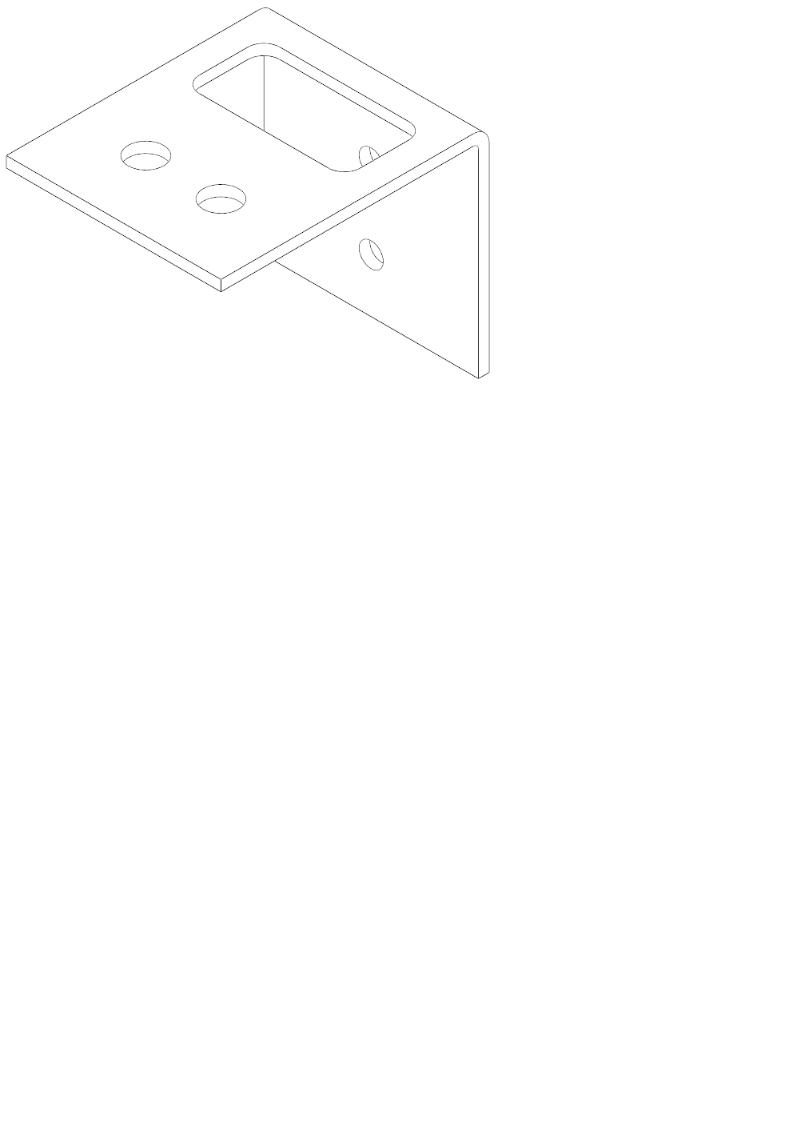
\includegraphics[width = 0.5\textwidth]{assets/figures/SupportChaineCable.svg}
    \caption{Représentation du support pour la chaîne porte-câbles}
    \label{fig:SupChaineCable}
\end{figure}

Deux passages de vis M4 sont présents pour la fixation sur le profilé ainsi que deux autres passages de vis M6 pour la fixation de la chaîne.
Un dégagement de matière est présent afin de pouvoir faire passer les câbles qui sortent de la chaîne et qui continuent plus bas vers le boîtier
électrique. Cette pièce est fabriquée en tôle pliée de 2~mm d'épaisseur et utilise un alliage d'aluminium différent, l'aluminium EN-AW 5052.\\

Un problème de soutien de la chaîne porte-câbles est survenu lors de l'assemblage. La description du problème et de la solution à appliquer
pendant le mois d'août est donnée dans le chapitre \ref{sec:ProbChaine}

\section{Plaque de passage pour moteur}\label{sec:PlaPassMot}
Afin de cacher l'arrière du système pour le rendre davantage présentable, mais aussi afin d'augmenter la rigidité du système, une plaque est placée
entre les deux profilés centraux. Les pièces faisant la liaison entre le moteur et le glider, décrites dans le chapitre \ref{sec:LiaisonMotGlid},
passent par cet endroit donc il faut découper une zone de passage pour ces pièces. Cela donne la plaque suivante.

\begin{figure}[H]
    \centering
    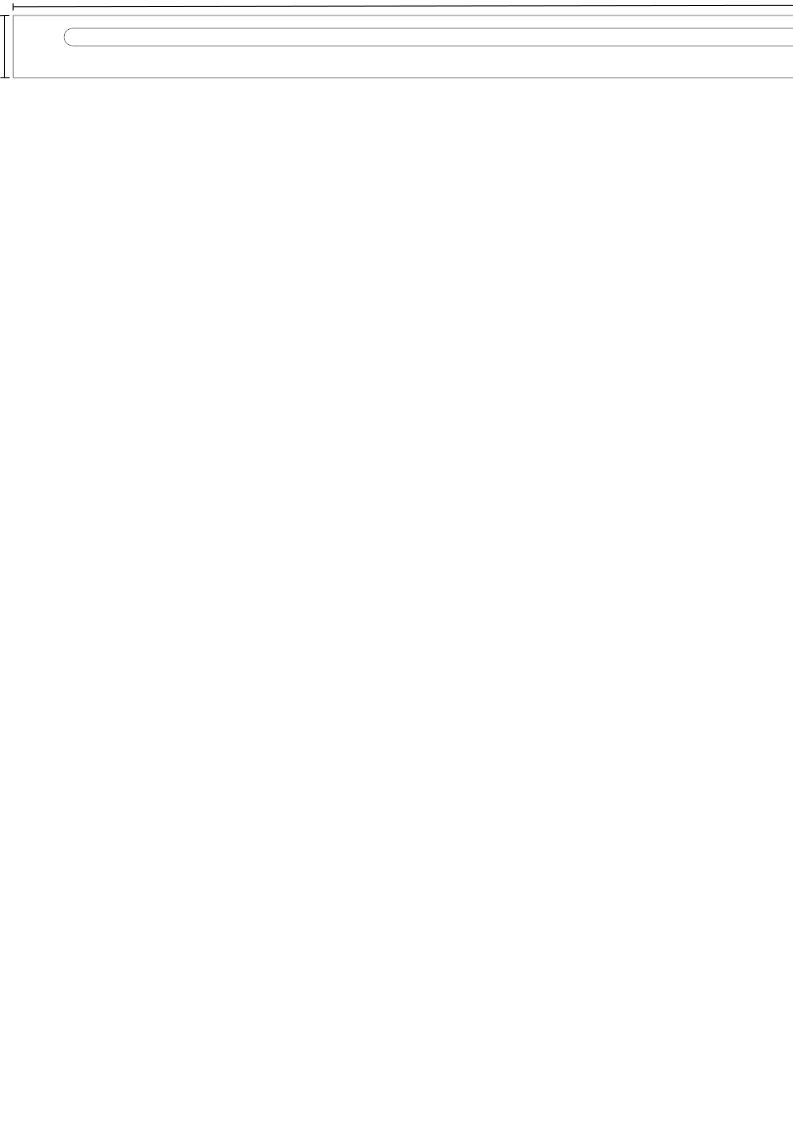
\includegraphics[width = \textwidth]{assets/figures/PlaquePassageMoteur.svg}
    \caption{Représentation de la plaque centrale}
    \label{fig:PLaPassMot}
\end{figure}

\section{Sécurité}\label{sec:Securite}
Une première sécurité qui a déjà été mentionnée dans le chapitre \ref{subsec:Amortisseurs} est constituée d'amortisseurs en bout de course pour
arrêter la partie mobile en cas de dysfonctionnement du pendule. Des arrêts d'urgence sont aussi présents afin d'arrêter manuellement le système
en cas de problème. Les arrêts d'urgence sont branchés directement sur l'alimentation 230~V du système donc la pression sur l'un d'entre eux coupe
immédiatement le système. Ceci à pour conséquence d'être néfaste pour l'électronique du système et peut corrompre l'OS de la carte RaspberryPi, il
faut donc utiliser ces boutons uniquement en cas d'urgence.\\

Une autre couche de sécurité viserait à empêcher les utilisateurs de pouvoir mettre leurs mains à des emplacements qui pourraient les blesser en
utilisant une plaque. La solution pensée est directement attachée aux supports des amortisseurs et viendrait se placer devant le rail ainsi que
les amortisseurs pour restreindre l'accès aux zones dangereuses tout en laissant l'accès à la tige pour la déstabiliser. Etant donné que la plaque
obstrue la vue d'une bonne partie du système, elle doit être faite d'un matériau transparent comme du \acrshort{PMMA}. Cette plaque n'a pas été
fabriquée pendant ce projet et sa mention n'est présente que comme recommandation pour l'utilisation du système lors de démonstrations publiques.
La figure suivante est une représentation hypothétique de la plaque et de son utilisation.

\begin{figure}[H]
    \centering
    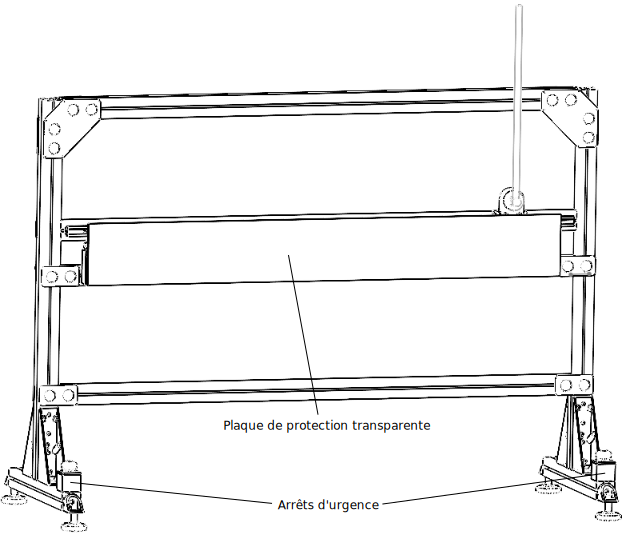
\includegraphics[width = 0.8\textwidth]{assets/figures/Securite.svg}
    \caption{Représentation des mesures de protections mises en place}
    \label{fig:Securite}
\end{figure}